%% LaTeX template for BSc Computing for Games final year project dissertations
%% by Edward Powley
%% Games Academy, Falmouth University, UK

%% Based on:
%% bare_jrnl.tex
%% V1.4b
%% 2015/08/26
%% by Michael Shell
%% see http://www.michaelshell.org/
%% for current contact information.
%%
%% This is a skeleton file demonstrating the use of IEEEtran.cls
%% (requires IEEEtran.cls version 1.8b or later) with an IEEE
%% journal paper.
%%
%% Support sites:
%% http://www.michaelshell.org/tex/ieeetran/
%% http://www.ctan.org/pkg/ieeetran
%% and
%% http://www.ieee.org/

%%*************************************************************************
%% Legal Notice:
%% This code is offered as-is without any warranty either expressed or
%% implied; without even the implied warranty of MERCHANTABILITY or
%% FITNESS FOR A PARTICULAR PURPOSE! 
%% User assumes all risk.
%% In no event shall the IEEE or any contributor to this code be liable for
%% any damages or losses, including, but not limited to, incidental,
%% consequential, or any other damages, resulting from the use or misuse
%% of any information contained here.
%%
%% All comments are the opinions of their respective authors and are not
%% necessarily endorsed by the IEEE.
%%
%% This work is distributed under the LaTeX Project Public License (LPPL)
%% ( http://www.latex-project.org/ ) version 1.3, and may be freely used,
%% distributed and modified. A copy of the LPPL, version 1.3, is included
%% in the base LaTeX documentation of all distributions of LaTeX released
%% 2003/12/01 or later.
%% Retain all contribution notices and credits.
%% ** Modified files should be clearly indicated as such, including  **
%% ** renaming them and changing author support contact information. **
%%*************************************************************************


\documentclass[journal]{IEEEtran}

\usepackage{graphicx}
% Insert additional usepackage commands here
\graphicspath{ {Figures/} }

\begin{document}
%
% paper title
% Titles are generally capitalized except for words such as a, an, and, as,
% at, but, by, for, in, nor, of, on, or, the, to and up, which are usually
% not capitalized unless they are the first or last word of the title.
% Linebreaks \\ can be used within to get better formatting as desired.
% Do not put math or special symbols in the title.
\title{ How Does Visualising Path-finding in an NPC Effect How Participants Explore a Level?}
%
%
% author name
\author{1507866}

% The paper headers -- please do not change these, but uncomment one of them as appropriate
% Uncomment this one for COMP320
\markboth{COMP320: Research Review and Proposal}{COMP320: Research Review and Proposal}
% Uncomment this one for COMP360
% \markboth{COMP360: Dissertation}{COMP360: Dissertation}

% make the title area
\maketitle

% As a general rule, do not put math, special symbols or citations
% in the abstract or keywords.
\begin{abstract}
The abstract goes here.
\end{abstract}

\section{Introduction}
% The very first letter is a 2 line initial drop letter followed
% by the rest of the first word in caps.
% 
% form to use if the first word consists of a single letter:
% \IEEEPARstart{A}{demo} file is ....
% 
% form to use if you need the single drop letter followed by
% normal text (unknown if ever used by the IEEE):
% \IEEEPARstart{A}{}demo file is ....
% 
% Some journals put the first two words in caps:
% \IEEEPARstart{T}{his demo} file is ....
% 
% Here we have the typical use of a "T" for an initial drop letter
% and "HIS" in caps to complete the first word.
\IEEEPARstart{T}{he} research question proposed in this project is: how does visualising \textit{Rapidly Exploring Random Trees} (RRT) path finding in a \textit{Non Player Character} (NPC) affect how a player explores a game level?


This project will look at visualising an enemy NPC's path-finding using RRT path-finding.   

Figure~\ref{KuffnerRRT} shows an example of RRT path-finding. Here the RRT explores the area and then draws a path along the tree~\cite{Kuffner2000}.  RRT involves nodes being randomly placed. Then it chooses a parent node based on whichever pre-existing node it closest to it.

This project will look at visualising the tree produced by RRT and the process taken to produce it.  The visualisation will be around an enemy NPCs. This will allow the participants to see where the enemy NPC is going and what their line of sight is. 

Implementation  of the visualisation will be in a level of a 3D game made in Unity 5.6~\cite{software:Unity}. Logging tools in the play testing software will record the amount of time spent in a level and what percent of the level they explore.   Analysis of this data will then determine whether the visualisation has any affect on participant exploration.

Previous papers have researched visualising~\textit{Artifical Intelligence} (AI) and foregrounding AI. However, there is little on on what effect this has on how the participants play the game.


\subsection{Hypothesis:}
\textbf{Null Hypothesis}: Visualising RRT path-finding has no affect on the percent of the level the participant explores. \\
\textbf{Hypothesis 1}: Visualising RRT significantly affects the percent of the level the participant explores. \\
\textbf{Hypothesis 2}: Visualising RRT significantly affects the length of time the participant spends in the level. \\
\textbf{Hypothesis 3}:  Visualising Unity navmeshes affects t  the percent of the level the participant explores compared to RRT. \\

\section{Related Work}
\subsection{Foregrounding and Visualising AI}
% Foreground visualising AI
Most modern digital game make use of AI.  However, it is rarely foregrounded or visualised in those games.   Treanor~\textit{et al} say that often the design of AI in games is to fit the game and complement game play. These AI are supporting the game play rather than being central to it~\cite{treanor2015}~\cite{eladhari2011}.  \\

Treanor~\textit{et al} surveyed many games that foreground or visualise AI in different ways.    From this they propose a series of design patterns for foregrounding AI in digital games. 
The two design patterns relevant to this project are ``AI as a Villain" and ``AI is Visualized" .  They describe the first pattern as having the AI not try to outright defeat the player. Instead it's designed to create an experience like in the game Alien Isolation~\cite{game:AlienIsolation, treanor2015}.  In Alien Isolation the AI hunts the player. This is foregrounding as the player has to observe the AI and learn how to avoid.  There is also some visualisation as the player has a scanner that will inform them of the AI's position. 

This paper will use ``AI as a villain" pattern as enemy NPC's  will have their path-finding visualized around them. The participants will have to observe this to learn how to not get caught by the enemy NPC.    


The second relevant design pattern is ``AI is Visualized".  This is where there is a visual representation of the AI's state or decision making in the game. 

Most games hide this from the player but this design pattern visualizes it making it mechanic.  
The example given by Treanor~\textit{et al} is the game Third Eye Crime.  Third Eye Crime is a game that followed the ``AI is Visualised" design pattern~\cite{Isla2014, game:ThirdEyeCrime}.  
The game uses probabilistic object tracking through Occupancy maps. The game uses Occupancy Maps to display where the enemy thinks the player could be in the map. As the enemy moves around the map it removes areas where the player is not from the Occupancy Map~\cite{Isla2014}.  

Generally stealth games involve avoiding enemies.  This design encourages the player to trigger the mechanic,  allowing them to use the visualisation to mislead and avoid the enemy~\cite{Isla2014}~\cite{game:ThirdEyeCrime}.  

This pattern is relevant to this project as the enemy NPC will have RRT path-finding visualized around it. Allowing the player to see where the enemy is going and decide how to overcome or outsmart it.

% Visualising in general
While Haworth~\textit{et al} do not visualise an AI decision making process they do visualise the possible decisions available to the player in a game on a tree structure~\cite{Haworth2010}.   They research visualising decision trees in a game to see what effect it had on children's analytical reasoning and game play.  
Their study did not come to any definite conclusions. However, their results suggested that the trees aided players. In the later levels of the game the children without the visualised decision tree struggled to beat the game.   However, they noted this could also be due to unbalanced later levels.  This makes the usefulness of the tree being questionable in this example.  

A potential issue with this study is that Haworth~\textit{et al} only tested the tree on a simple 2D game for school children. Of these school children only a few had experienced playing digital games before.  This may mean that this data may not be relevant for 3D games or games available to buy on the market.  In contrast, Isla's visualised Occupancy Maps are in the game Third Eye Crime which is available on Steam, IOS and Android~\cite{Isla2014}~\cite{game:ThirdEyeCrime}.

Like  Haworth~\textit{et al}, Bauer~\textit{et al} also research visualising tree structures~\cite{bauer2012}. However, they did use an AI technique, they used Rapidly-Exploring Random Trees (RRT).

Another use of visualisation is in game design. Often to check player behaviour in player testing or to aid the design of levels~\cite{Nelson2011}~\cite{bauer2012}~\cite{Tremblay2013}~\cite{Tremblay2014}. 


\subsection{Pathfinding}
% A* / pathfinding in games
In digital games the A* path-finding algorithm appears to be the most used~\cite{Algfoor2015}.  Algfoor~\textit{et al} surveyed numerous papers on path finding. 

Their focus was on the use of different grids in path-finding and the numerous algorithms available~\cite{Algfoor2015}. The most popular being the A* algorithm for use in both digital games and robotics. RRT path-finding was not mentioned here. 
They surveyed many grid types and gave the advantages of each. However, RRT does not use grids it instead uses nodes making the grid type irrelevant.

Hu~\textit{et al} propose an implementation of A* path-finding in the Unity engine, the engine used in this project~\cite{Hu2012}.  While their implementation is in an older version Unity the implementation in Unity 5.6 should still be similar. 

The previous section mentioned Third Eye Crime for it's foregrounding of AI.  It also uses visualisation as an important mechanic~\cite{Isla2014}~\cite{ game:ThirdEyeCrime}.  Isla uses Occupancy Maps to show where the enemy NPC thinks the player could be. Occupancy or Influence maps do not produce a path instead they show the probability of the player being in different locations across the map~\cite{Isla2014, Miles2006}. Isla used Occupancy maps to show where the enemy AI thinks the player currently is. The enemy then moves to investigate that area reducing the probability of the player being there to 0.  Similarly, Miles and Loius used also used influence maps. While their example is specific to \textit{Real Time Stratedgy} (RTS) games, like Isla they used Occupancy maps.  They used them as a base to for A* path-finding instead of A* using the map itself for path-finding~\cite{Miles2006}.\\

A further paper on path-finding is Wang and Lu's paper which looks at path-finding in a 3D environment. While again they were using A* they look at using A* in 3D and suggest using nodes instead of a grid~\cite{wang2012}.

Mendonça~\textit{et al} look at path-finding both in robotics and digital games~\cite{Mendonça2015}. Their focus is on stealth path-finding in games and applying that to robotics. Like RRT, the methods they propose does not necessarily find the optimal path~\cite{karaman2010}~\cite{Mendonça2015}. Instead they try to find the most stealthy path. They generate custom navigation meshes (navmeshes). Then they assign a weight to each polygon in the navmesh depending on how close it is to being behind cover. 

As Mendonça~\textit{et al} use path-finding to find a stealthy path, the path with the optimal distance may not always be the path with the lowest cost in relation to the AI agent being in cover. Therefore, a requirement might not always be the optimal path. 

This project will favour interesting visualisations over the optimal path in the variants that use RRT. 

%^^ point is optimal not always necessary ^^

%  RRT
Rapidly-Exploring Random Trees~(RRT) are a search method used more in robotics than digital games~\cite{LaValle1998}~\cite{Kuffner2000}.   Kuffner and LaValle first proposed RRT. They intended to produce a random algorithm more efficient than the other search algorithms available at the time. 

Figure~\ref{KuffnerRRT} shows  Kuffner and LaValle's RRT Path Planner. Path Planner is a variant of RRT which has the intended use of finding paths from a generated tree~\cite{Kuffner2000}.
\begin{figure}[h]
	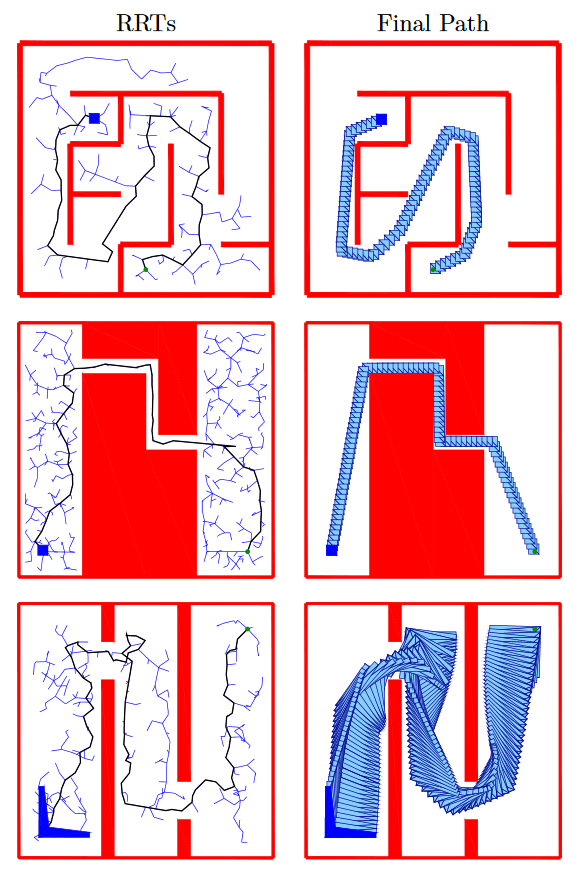
\includegraphics[width=1.0\linewidth]{KuffnerRRT.png}
	\caption{ Kuffner and LaValle's \cite{Kuffner2000}.}
	\label{KuffnerRRT}
\end{figure} 

RRT's goal is to find a path between two point with no collisions. The path found may not be the optimal path though~\cite{Kuffner2000, Karaman2011}.  Karaman and Sertac say that the chance of RRT finding an optimal path is very unlikely~\cite{karaman2010}~\cite{Tremblay2014}.  Karaman \textit{et al} propose a variant of RRT called RRT*. RRT* starts the same as RRT. However, when a new node has to choose a parent node instead of choosing the  nearest node it evaluates the cost of the nodes in regards to reaching it's goal. Each iteration involves re-evaluating parent nodes to reduce the cost. Rewiring of the tree happens when a lower cost path is located.

%  RRT & games
Bauer and Popovic use RRT for level design in digital games~\cite{bauer2012}. Like Haworth \textit{et al}, they visualise the data to aid users~\cite{bauer2012}~\cite{Haworth2010}. However, unlike Haworth \textit{et al} the visualisation is for game developers not the players. 

\begin{figure}[h]
	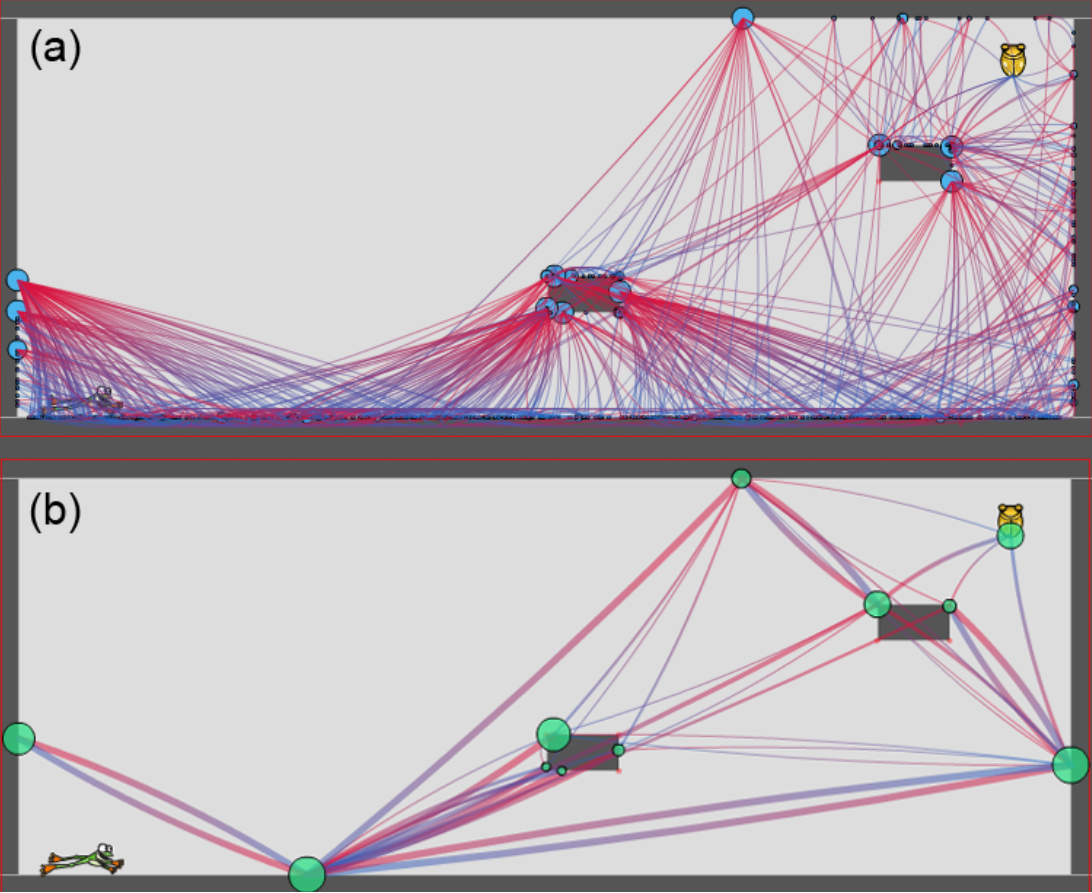
\includegraphics[width=1.0\linewidth]{BauerRRT.png}
	\caption{ Bauer \textit{et al}'s graph-based representation of RRT with and without clustering \cite{bauer2012}.}
	\label{BauerRRT}
\end{figure} 

Their focus is on level design not game-play. They propose a tool that analyses a level generated by PCG or a level designer. They then use RRT to calculate possible routes the player could take when playing.  
This produces an image that is difficult to read. The use of Dongen's method for graph clustering makes the output more legible~\cite{bauer2012, van2001}.  

The focus of this project is on a similar type of  visualisation but in a game instead of game design. Therefore, there is a need for a similar technique to organise the output of RRT.  This should make the visualisation  more useful as it should aid the player in way that they can look at the visualisation and interpret what the NPC is going to do. 


Tremblay~\textit{et al}, like Bauer and Popovic, also use RRT visualisations to aid level design~\cite{Tremblay2013}~\cite{bauer2012}. 

Like Mendonça~\textit{et al}, they focus on designing stealth games and finding stealth orientated paths in the game levels~\cite{Mendonça2015} \cite{Tremblay2013} . Like Bauer and Popovic, they use RRT to visualise possible moves the player could make. Then they use clustering to make the results less cumbersome to the user~\cite{Tremblay2013}. 

The use of RRT in this case is because it is flexible and inexpensive. Also it's random nature mirrors a wide range of player behaviours~\cite{Tremblay2013}. 
This project will use RRT but not for reflecting player behaviour.  Instead it's use  is for creating a visualisation that fits with the game and that is interesting for the player to interact with. A path that is interesting to play with is more important in this project than an optimal path. There will then be a comparison between a visualisation of the Unity navmeshes against the RRT visualisation.

While the use of RRT to find a stealthy path is different to it's use in this project a potential problem is that Tremblay~\textit{et al}'s results showed that the chances of their RRT implementation finding a path decreased as the grid size increased. It also decreased as the number of attempts decreased as shown in Figure \ref{TremblayRRT}. 

% EXPAND ON POTENTIAL ISSUE WITH IT RUNNING ONCE

\begin{figure}[h]
	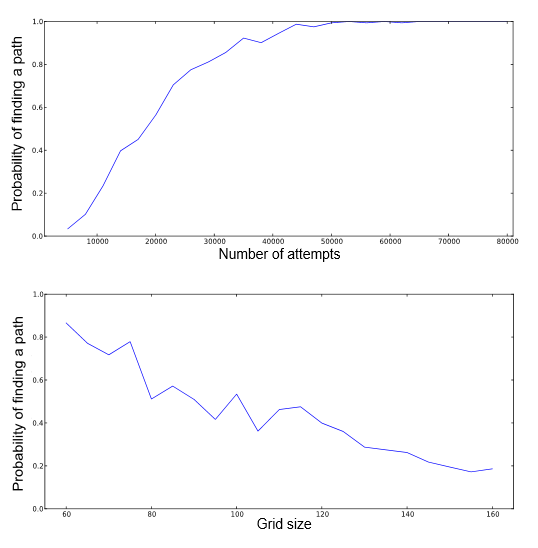
\includegraphics[width=1.0\linewidth]{Tremblay2013.png}
	\caption{ Performance analysis of Tremblay~\textit{et al}'s RRT when running on a Metal Gear Solid level~\cite{Tremblay2013}~\cite{game:MetalGearSolid}.}
	\label{TremblayRRT}
\end{figure} 

\begin{figure}[h]
	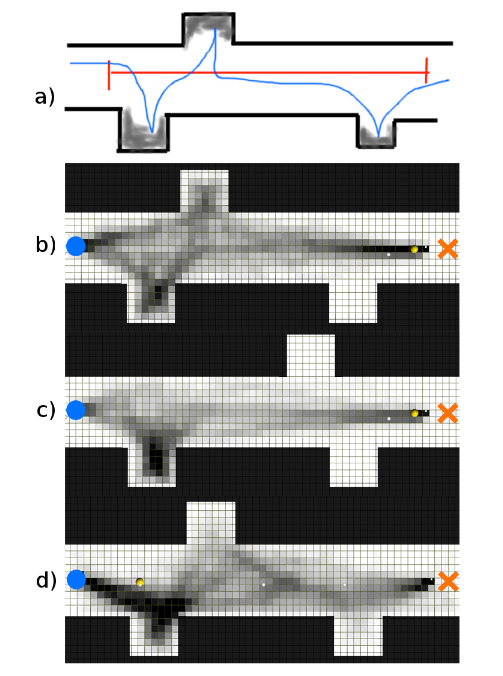
\includegraphics[width=1.0\linewidth]{TremblayHeatMap.png}
	\caption{ Heat maps of a single level where the design has been changed each time \cite{Tremblay2013}.}
	\label{TremblayHeatMap}
\end{figure} 

Tremblay~\textit{et al} again look at the use of search algorithms for use in game development. This work builds on the 2013 paper on RRT in stealth games~\cite{Tremblay2014}. They look at the use of A*, \textit{Mote Carlo Tree Search} (MCTS) and RRT to visualise player behaviour in platform games similar to Bauer ~\cite{Tremblay2014}  ~\cite{bauer2012} . 

RRT is limited to drawing straight lines between the nodes, as straight lines are not always possible in RRT  Tremblay~\textit{et al} also use either A* or MCTS to find a path to the node and ensure that it is reachable.
% EXPAND ON

\begin{figure}[h]
	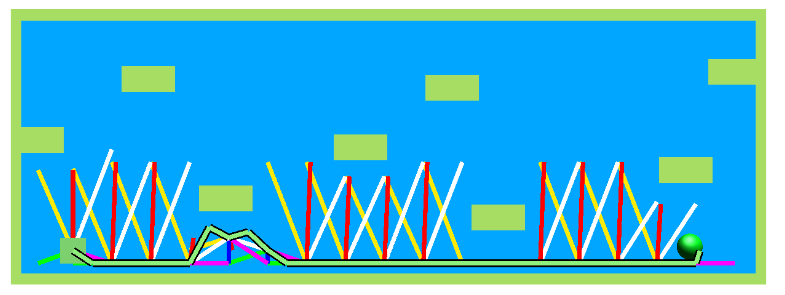
\includegraphics[width=1.0\linewidth]{Tremblay2014.png}
	\caption{ Tremblay~\textit{et al}'s visualisation of an RRT tree~\cite{Tremblay2014}.}
	\label{Tremblay2014}
\end{figure} 

% RRT vs  A*
% A* and optimal paths vs RRT better visualisation 


\subsection{Exploring Game Environments}
% Wayfinding
One method of guiding players through games is to use way-finding. Way-finding in games is often visual cues in the environment that will guide the player to an area of interest~\cite{si2017, Bacim2008}. 

The intention of visualising RRT path-finding in this project is not to guide the players. However, like Si \textit{et al}  it will observe how players navigate and explore levels and whether, like the presence of way-finding cues, it affects player behaviour. 

Moura and Bartram investigate the effects of different way-finding cues on players~\cite{moura2014}.  They looked at methods used in triple A games and mimicked them in their own game. Their results show that the absence of way-finding cues was obvious to players. In contrast, the version with way-finding cues did not have enough cues to sufficiently guide the player. These results suggest that way-finding cues alone may not be enough to guide the player. While the use of visualisation of RRT path-finding in this project will be as an enemy another application could be in way-finding. Either as an enemy or friendly NPC the visualisation of path-finding could have a use a an aid to the player. However, Moura and Bartram concluded there is a need for more research as the results were inconclusive. 
 
% Player Exploration
Si \textit{et al} investigated how players explore virtual environments~\cite{si2017}. While their experiments were specific to Real Time Strategy (RTS) games the results may apply to other game types. Si~\textit{et al} say that three common types of spatial exploration are; environment mapping, bonus item collecting and location/landmark discovery. The relevant exploration type for this project is spatial mapping. Firstly as it is what the enemy NPC will be doing.  Secondly as it is the player behaviour that is being measured by the logging tool in the software.

Haworth~\textit{et al} did not look at player exploration but the game they used in their study involved a map where participants had to explore a maze. Participants which had the decision tree visualisation found it easier to navigate the maze. This suggests that visualisation could aid the exploration process~\cite{Haworth2010}.

\section{Methodology}
The methodology that will be used to test the given hypothesis will be play testing and questionnaires. This will require human participants to play the game and fill in the questionnaires. 

The game the enemy NPC will be tested in is a 3D metroidvania game which has a focus on exploration. Players will be given one of the game variations to play and then asked to complete a questionnaire on their experience. The game will also log the players position at regular intervals to calculate what percent of the level they explore. How long a participant spends exploring the level will also be logged.  

\subsection{Playtest Variations}
There will be multiple variations of the game to test the different hypothesis. 

\subsubsection{Control: Unity Navmesh}
The first variation will be the control version of the game. This version will have no visualisation on the enemy NPC's path-finding. The enemies in the game will use the default Unity navmeshes.

\subsubsection{Unity Navmesh Visualised}
The second variation use Unity's built in navmeshes and navmesh agents for path-finding. This will be visualised on the floor of the level around the enemy NPC.

\subsubsection{RRT Path-finding Visualised}
The third variation will have visualised path-finding. The path-finding will use RRT and the player will be able to see three around the enemy NPCs.

\subsubsection{RRT path-finding}
The final version will also use RRT path-finding but there will no visualisation around the enemy NPC.

A-B testing will used on participants. A-B testing is where each participant will be assigned a version of the game to play~\cite{Hynninen2014}. In this case to prevent them from working out what the goal of the play test is. 
\\
The software will log the participant's position in the level throughout their play test. This data will be exported in a .CSV every second. Varying the export rate is unlikely to provide data of interest as the focus is on time spent in a level and how much was explored. 

The exported data will then be analysed using R. Wallner says heat map are useful as they are easy to generate and easy to discern patterns from~\cite{Wallner2015}.  Tremblay~\textit{et al} also used heat maps on their RRT visualisations. They used heat maps as part of their tool for level designers to use to see where player could go and the effects of them altering the level design which can be seen in Figure \ref{TremblayHeatMap}. Here they will only be used for analysis and to assist in finding noticeable patterns.
\\
Other statistical analysis in R, such as bar charts, will also be generated to support the heat maps.
 
After completing a play test of the game participants will be asked to complete a questionnaire on their experience.\\

\subsection{Questionnaire}
Alongside play testing participants will also be asked to fill out a questionnaire on the game online using Google Forms. Nordin \textit{et al} say that questionnaires are vital for understanding how players feel when playing digital games~\cite{nordin2014}~\cite{Denisova2016}. They can also help give uniformity and consistency to the data gathered from participants~\cite{Denisova2016}.

Questionnaires are also beneficial as they can prompt players to give answers they may not have given spontaneously. The two options here are to either create a questionnaire specifically for the experiment or use an existing one. There are a wide variety of questionnaires that already exist to measure players experiences in play testing~\cite{nordin2014}~\cite{Jennett2008}. These come with the benefit of being more likely to be thoroughly tested such as the \textit{Immersive  Experience
Questionnaire} (IEQ) which uses Likert scales responses~\cite{nordin2014}~\cite{Jennett2008}.
 
However, Nordin \textit{et al} say there are many issues with using existing questionnaires. Firstly, many of these questionnaires are not readily available. Another issue is that not all questionnaires have been thoroughly checked for validity. There is the potential issue of a researcher not fully understanding the questions put forward by another researcher or may not understand what data that question is intended to get.

As the quantitative data gained from play testing is more important than qualitative data here the questionnaire will be based on the IEQ with added questions related to the visualisation. The IEQ tests for immersion but has questions related to interacting with the game world and causes of frustration in it that may relate to the visualisation of path finding.



\section{Conclusion}
In conclusion, while the use of RRT's is more frequent in robotics than digital games it's use appears feasible in this project. It's past use in game design tools shows that clustering can make the output understandable to the user. However,  the need of optimisations  such as RRT* or the use of A* may arise to produce of more optimal path. 

Visualisation and foregrounding of AI has been successfully used before again suggest it can used here. Finally previous studies have looked at way-finding and player exploration. These suggest that environmental factors in digital environments do affect player exploration.
% references section

\bibliographystyle{IEEEtran}
\bibliography{references}

% Appendices

% \appendices
% \section{First appendix}
% Appendices are optional. Delete or comment out this part if you do not need them.

% that's all folks
\end{document}
